\chapter{Simulating Human Agents for Testing HAN}
One of the challenges during the development of a HAN system is to test the system before its final deployment and real-world runs. Robotic simulators are of great use during this period as we can test the system under various conditions and in several environments. Unlike the classical setting, testing HAN requires the simulation of humans, which is still research under development. Until recently, the HAN community used the crowd simulators like Pedsim or MengeROS~\cite{aroor2017mengeros} to simulate humans in semi-crowded or crowded scenarios. However, the motion generated by these simulators uses reactive schemes like \acrshort{sfm} or \acrshort{orca}, which are good for generating crowds but lack intelligence at the level of an individual human. Recent simulators like SEAN~\cite{tsoi2020sean, tsoi2022sean} and SocNavBench~\cite{biswas2022socnavbench} tried to generate somewhat intelligent behaviours using new approaches and real-world data. However, these human agents are either not reactive (as they replay real-world trajectories without considering the robot) or use schemes similar to \acrshort{orca}. Although they have better human agents and environments for testing HAN, they still lack intelligent agents that can be used to test intricate scenarios in spaces like offices, labs or homes. Hence, we have used different ways to control the human(s) while testing the HAN proposed in this thesis. These ways include manual control using a joystick, a simple human controller that follows the generated trajectories, and finally, an intelligent human with rational decision-making capabilities.      

\section{Planning and Control for Human Agents}
In this section, we talk about the simple modes and planners employed to control the human avatar in the robot simulator. A human is assumed to be a robot with special requirements.

\subsection{Manual Control}
One of the simplest ways to control a human is to move the human manually using a keyboard or joystick. This is efficient in testing some very complicated scenarios involving intelligent decisions. Since a real human is already controlling the human avatar in the simulator, all the decision-making process is handled by the human operator. To integrate such human avatar into our system, we used the \textbf{\textit{joy}}\footnote{\url{http://wiki.ros.org/joy}} \acrshort{ros} package and then mapped the inputs of the joystick to the avatar's velocity with a cap at \SI[per-mode=symbol]{2}{\metre\per\second}.

Manual control is good for testing some interesting and particular cases, but it becomes tiresome to run several scenarios to benchmark or quantify the results. Moreover, the simulation runs cannot be completely automated as the human operator is always involved in the loop. So, the next solution was to plan and control the human, like the robot. It is different from collision avoidance algorithms as the human has a global path to trace and a separate local planner to move the human. 

\subsection{Planning based Control}
To automate and replicate the tasks easily, we have developed a simple \textbf{\textit{humans navigation}}\footnote{\url{https://github.com/sphanit/humans_nav}} package using the \textbf{\textit{global planner}}\footnote{\url{http://wiki.ros.org/global_planner}} in \acrshort{ros} and a simple controller. The developed system has two modes of operation:
\begin{enumerate}
    \item \textit{Trajectory following}: In this mode, the human follows the trajectory that is provided externally through a \acrshort{ros} topic. We used this mode to test the ideal situations where the human follows the trajectory planned by \acrshort{cohan}.
    \item \textit{Goal-based Control}: This mode is more autonomous as we only provide a goal via a \acrshort{ros} topic, and the system plans and moves the human to the goal. The planning module updates the plan as the human moves, and the simple controller traces the path. This mode was used to run multiple tests to check how well the robot adapts to the human.
\end{enumerate}
Both these modes can control more than one human simultaneously. The \textit{Trajectory Following} mode used the trajectories planned by \acrshort{cohan} to move the humans. The trajectory provided the desired velocities, which were sent directly to the human controller. However, in the \textit{Goal-based Control} mode, the velocities were calculated based on the current position and planned paths of the humans. To accept multiple goals and plan for all the humans together, a \textbf{\textit{multi-goal planner}} was developed, and it is used internally by the \textbf{\textit{humans navigation}} package to get plans based on the provided goals.

Even though this kind of system solves the issues of automation and is less tiresome to the developer, the human agent is still not intelligent and simply follows the given trajectory. Although the trajectory provided by \acrshort{cohan} takes care of many human-robot social constraints, this ideal behaviour may not be expected from humans. In the second mode of control, the human agent might have better behaviour, but the agent is still not intelligent and somewhat reactive, like in collision avoidance schemes. 

\section{InHuS}
InHuS\footnote{\url{https://github.com/AnthonyFavier/InHuS_Social_Navigation}}~\cite{favier2022_hri} stands for \textbf{I}ntelligent \textbf{Hu}man \textbf{S}imulator, and it was developed to specifically simulate a human agent that is rational and persistent about its goal, unlike the reactive schemes. 
\begin{figure}[!hb]
    \centering
    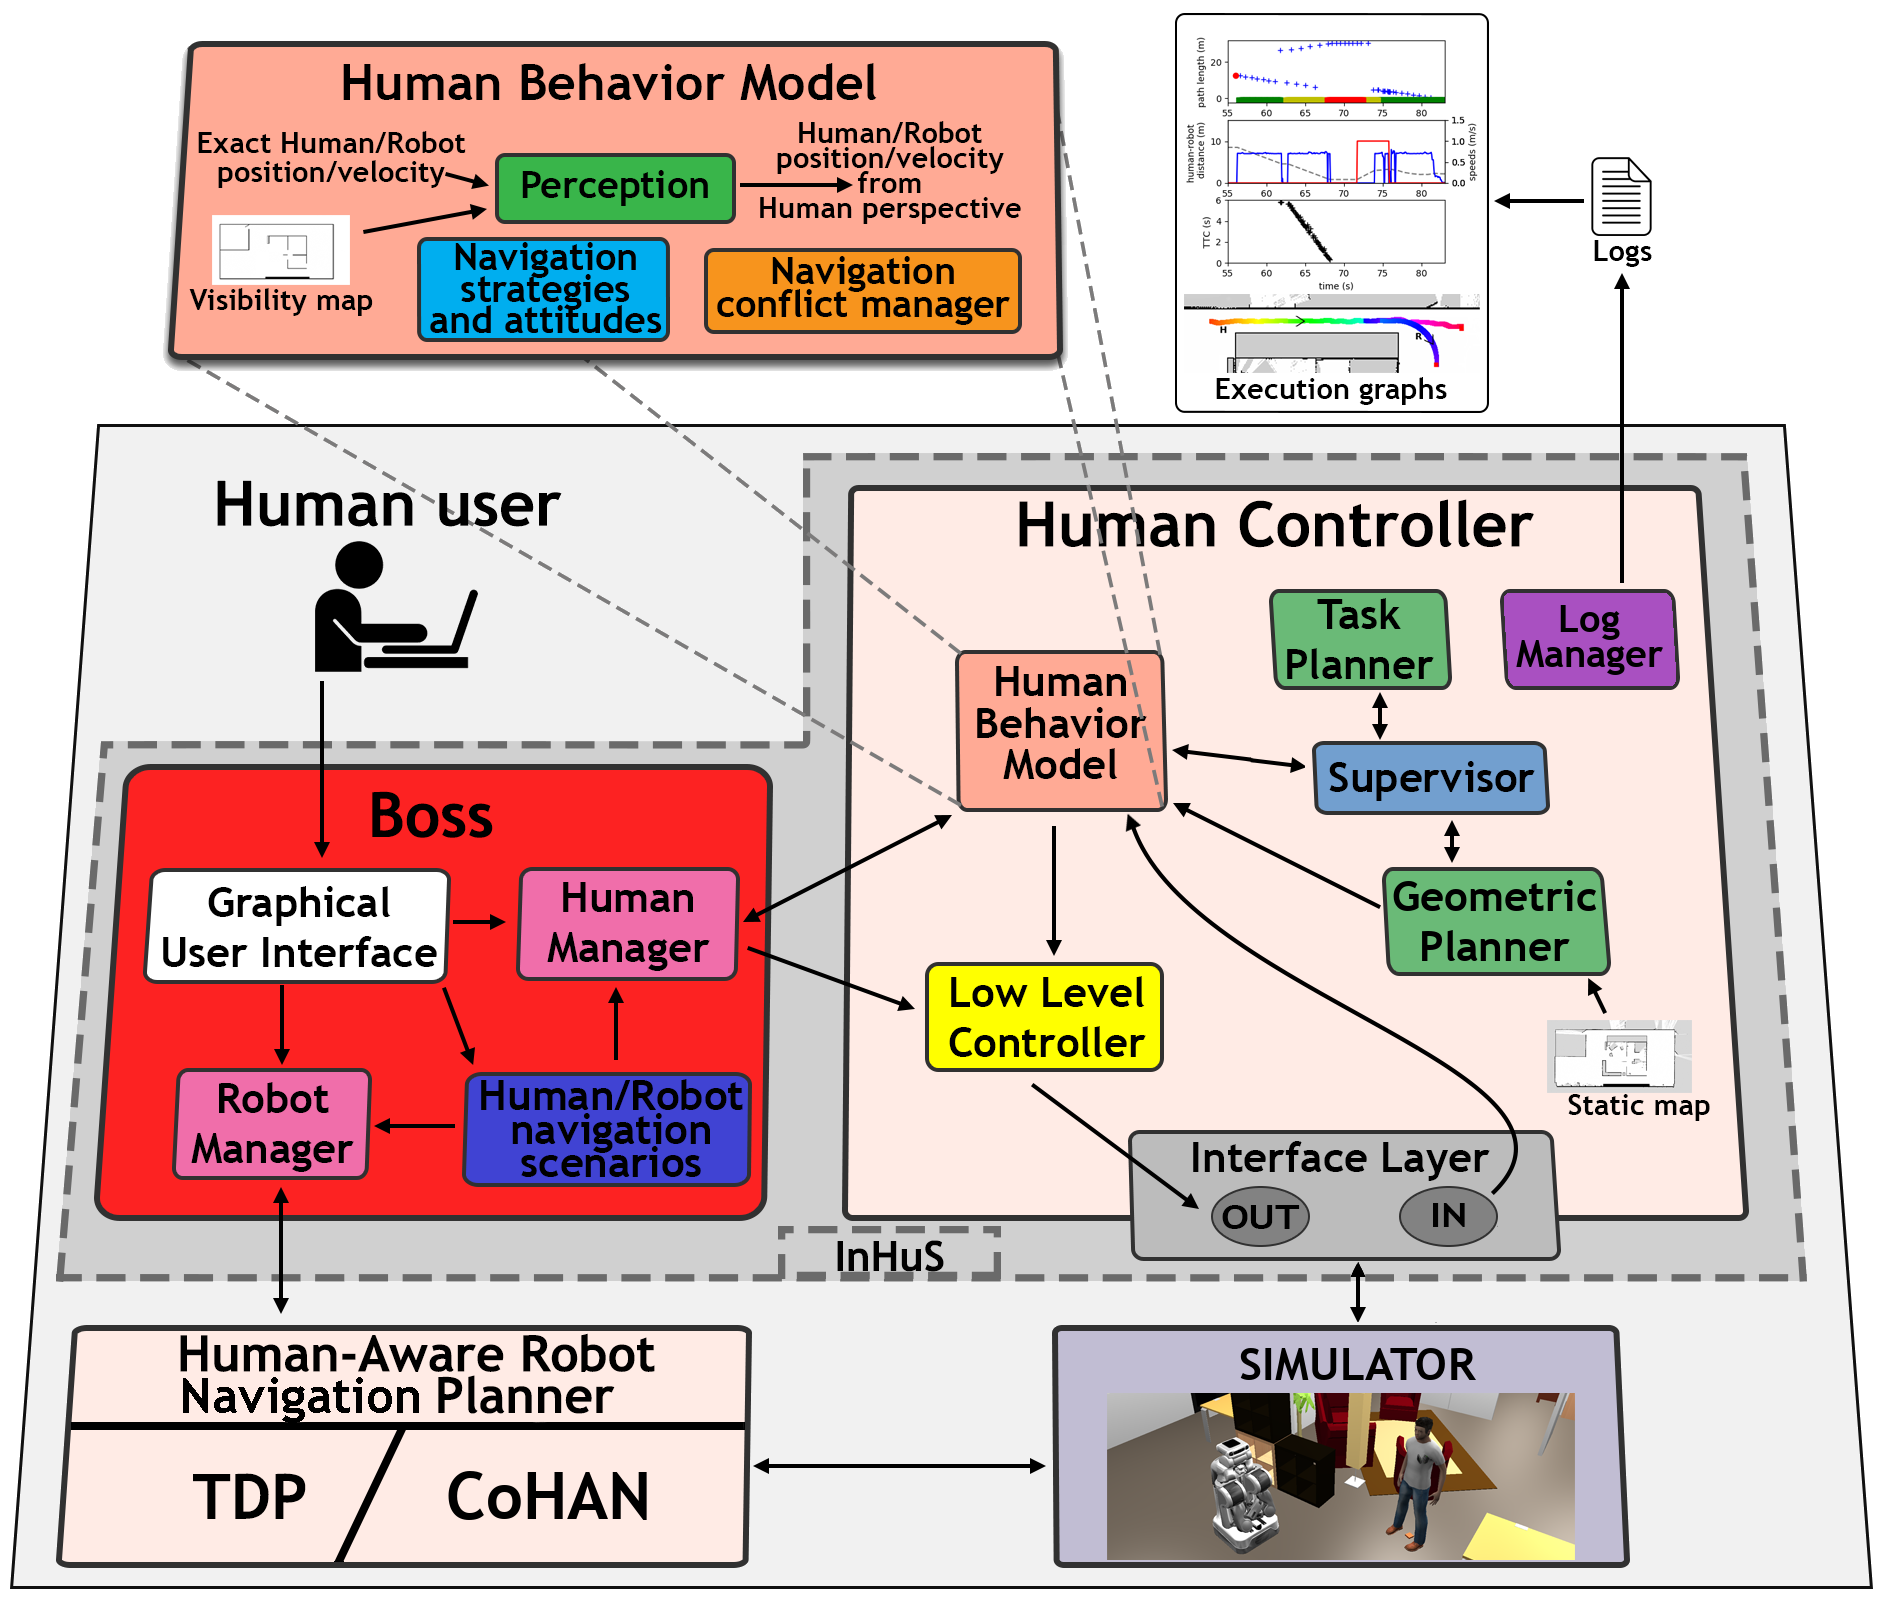
\includegraphics[width=0.9\columnwidth]{images/appendix/architecture.pdf}
    \caption{InHuS Architecture. The system consists of the Boss and the InHuS Human Controller macro components. The human operator interacts with the system through the Boss which in turn interacts with the Human Controller and the HAN Planner. Both the human and the robot controllers are connected to the same simulator where they control different components but share the same environment.}
    \label{fig:inhus}
\end{figure}
\subsection{Architecture}
The architecture of the proposed system is shown in Fig.~\ref{fig:inhus}. InHuS is composed of two major components namely, 1) \textit{Boss} and 2) \textit{Human Controller}. These components are explained in detail below:
\begin{itemize}[label={}]
    \item \textbf{Boss}: The \textit{Boss} component is responsible for taking input from the user and sending the appropriate instructions to the human and the robot planners. Hence it is provided with a graphical user interface through which a user can give individual goals to each agent, run or re-run predefined scenarios or initiate an endless loop of the human and robot navigating continuously from one goal to another. The endless loop can be used to identify the limits of the HAN system under test. After taking the input from the user, this component communicates the navigation goals to the \textit{Robot Manager} and \textit{Human Manager} at the appropriate times. Once the goals are communicated to these components, the \textit{Boss} does not interfere with the execution unless the human operator selects a new goal or scenario.
    \item \textbf{Human Controller}: This is the main component of InHuS that controls human motion and decides what to do in case of a conflict with the robot. It has an internal `\textit{Human Behaviour Model}' that makes these decisions and sets some attitudes to humans. The other major sub-component is the `\textit{Supervisor}', which supervises the execution of the goal and the progress, and activates the respective components as needed. While the `\textit{Geometric Planner}' provides the geometric path and trajectory to the goal, the `\textit{Low Level Controller}' sub-component sends the command velocity to the human avatar. The `\textit{Task Planner}' was used to define different kind of navigation tasks like \textit{go to goal}, \textit{wait} etc. Finally, the \textit{Log Manager} of this component logs the data and sends it to a GUI for visualisation of the calculated metrics.
\end{itemize}

\subsection{Supervisor and Geometric Planner}
The navigation goal of the human avatar is sent to the \textit{Supervisor}, which in turn asks the \textit{Task Planner} for a plan to achieve this goal. The \textit{Supervisor} then supervises and coordinates the execution of all the actions in the plan while managing the conflicts. The navigation plan generally consists of `moving' and `waiting' actions. This kind of architecture allows us to define complex navigation goals with multiple steps. The \textit{Supervisor} queries the \textit{Human Behaviour Model} from time to time to detect any potential conflicts. It has the power to suspend the execution of a plan in case of a conflict and resume it whenever necessary. This is especially useful to execute other actions in case of conflict to show the navigation intention and goal persistence of the human agent, unlike the reactive or simple planning approaches.

When the \textit{Supervisor} has to execute a `moving' action, it sends the navigation goal to the \textit{Geometric Planner}, which generates the path and then calculates the velocity commands to make the human move towards the goal. Depending on the type of trajectory planner selected, human motion can be different. In the current version, the standard \acrshort{ros} Navigation Stack or \acrshort{cohan} can be selected as the \textit{Geometric Planner}. The velocity command given by this component is not directly sent to the human. The \textit{Low Level Controller} receives this velocity and, if necessary, modifies or perturbs this velocity before sending it to the human avatar. This is used to emulate some reactions while navigation called `\textit{Attitudes}', which is presented in the next subsection.

\subsection{Human Behaviour Model}
The \textit{Human Behaviour Model} is the most important component of the proposed architecture. It controls the human avatar and is responsible for the behaviours exhibited by the human agent. As mentioned previously, this component manages the navigation conflicts, and in this version, only the blockage of the path by the robot is handled. Whenever the \textit{Geometric Planner} is called for the first time, the shortest path to the goal without any moving agents is calculated and sent to the `\textit{Navigation Conflict Manager}' of this component. If any blockage of this path by the robot is detected by this component, it changes the human state, and then the \textit{Supervisor} suspends the goal. The human avatar then performs an `approach' action where it moves towards the goal until it reaches a limiting distance from the robot. After this, it stops and waits for the robot to clear the way. Note that any collision avoidance or simple planning strategies will fail to show such behaviour as they will completely change the path of the human agent instead of showing persistence towards the goal.

This component can also set the goals for the human agent apart from the \textit{Boss}. The internal goal selection mechanism is responsible for different \textit{Attitudes} of the human avatar. Three kinds of attitudes are provided in InHuS:
\begin{enumerate}
    \item \textbf{Stop and Look}: It emulates a curious behaviour, where the human avatar navigating to the goal stops and looks at the robot shortly if the robot is in close vicinity of the human avatar. After this action, the navigation to the original goal is resumed.
    \item \textbf{Harass}: This attitude emulates a behaviour where the human avatar continuously disturbs the robot by blocking the robot's path. The idea here is to generate a child-like behaviour for the human avatar.
    \item \textbf{Random Goal}: In this attitude, a new random goal is set to the human avatar while it is already moving towards a goal, emulating something like a change of mind.
\end{enumerate}
To make the system more realistic, this module builds the perception of the human avatar using the map of the environment and the location of the other agents. The information about the other agents is taken directly from the simulator rather than using simulated cameras or lasers. Therefore, the human avatar does not consider the robot that it cannot see, even if it is below the threshold distance geometrically.

\subsection{Logs and Metrics}
The \textit{Log Manager} logs the data of the human-robot navigation interactions and sends it to GUI based data visualiser. This visualiser shows the different states of the human, the paths of the human and the robot, and some metrics to evaluate the robot's navigation. The logged data can also be used to calculate new metrics or methodologies for evaluation. A screenshot of this visualisation is shown in Fig. \ref{fig:gui_inhus}.
\begin{figure}[!ht]
    \centering
    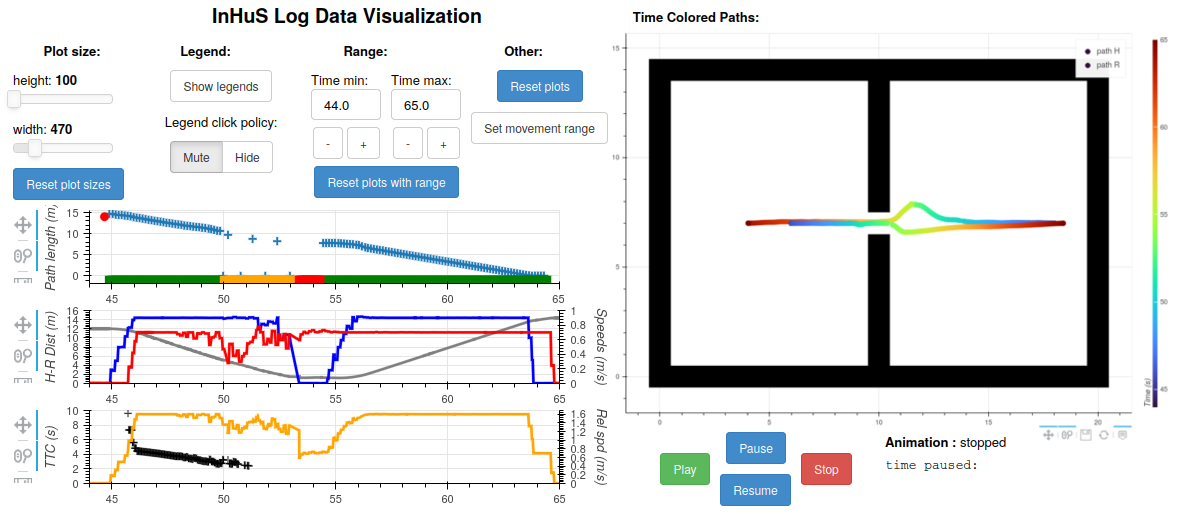
\includegraphics[width=0.9\columnwidth]{images/appendix/gui_bis_bis.png}
    \caption{The data visualisation in GUI. On the right, the paths taken by the agents are shown, while on the left, the human states and the calculated metrics are shown.}
    \label{fig:gui_inhus}
\end{figure}
The paths shown on the right in Fig. \ref{fig:gui_inhus} are coloured over time. It means that the same colour on the paths represents the same time instant, and using this, one can interpret the behaviour of the agents better. On the left, the plot on the top shows the human avatar's distance to the goal and its estimated state over time. If no conflict occurs, the human stays in a single state, and the distance to the goal decreases linearly. The plots below the first one show some of the calculated metrics and the agents' velocities over time. One can calculate and add more metrics as needed using the logged data.

\subsection{Generating Different Behaviours}
\begin{figure}[!h]
    \centering
    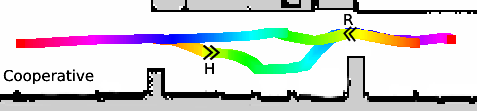
\includegraphics[width=0.9\columnwidth]{images/appendix/paths_coop_new.png}
    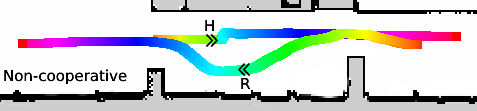
\includegraphics[width=0.9\columnwidth]{images/appendix/paths_stop_new.png}
    \caption{Traversed paths generated by InHuS during the Pillar corridor scenario. The top part is with cooperative settings and the bottom part with non-cooperative settings along with the \textit{Stop and Look} attitude.}
    \label{fig:paths_pillar_corridor_inhus}
\end{figure}
Depending on the \textit{Geometric Planner} and the \textit{Attitude}, different navigation behaviours can be emulated for the human avatar. For example, using the standard \acrshort{ros} Navigation stack and \textbf{Stop and Look} attitude, we can simulate a non-cooperative human who contributes nothing in a setting like a corridor. If \acrshort{cohan} is used, a cooperative yet curious human can be simulated. Moreover, \acrshort{cohan} can be tuned to set a degree of cooperative behaviour. The comparisons of different combinations and behaviours generated are presented in more detail in \cite{favier2021simulating}. Fig. \ref{fig:paths_pillar_corridor_inhus} shows the paths of the robot and human in two situations, one where the human is non-cooperative and curious and the other in which the human is completely cooperative.

% \section{ImHuS}
